% 附录 Y：强场与激光等离子体（v1.23.0 新增）
% 数值唯一来源：tools/calc/appY_calc.py -> tools/calc/appY_calc.txt（正文数字的唯一来源；检查项 P30）
% 长度/功率单位写成 cm、TW，避免中文字符进入数学字体；全部数字可用仓库脚本复算。
% 版权口径：只借鉴经典教材与文献的物理结论、公式形式与题型；文字、数值与表格自拟并独立复算。
% 本书不列 DOI，只给书名、作者、年份、卷期页。
% 分工：M 管加热与电流驱动，N 管边界与瞬态热负荷，S 管约束，U 管增益与点火，
%       V 管运行空间什么时候被撞破，W 管快粒子与 alpha 粒子，X 管辐射这条出口；
%       本附录管另一个极端——激光场强到电子在一个周期内就被推到近光速时会发生什么。

\section{三个刻度：场强、功率与压强}
\label{sec:app-y-scales}

前面所有附录都活在磁约束的世界里：磁场几特斯拉、温度几 keV、密度 $10^{20}\ \mathrm{m^{-3}}$。
本附录换一个极端。强场激光等离子体的电场是 $10^{14}\ \mathrm{V\,m^{-1}}$ 量级，
功率密度比托卡马克的加热功率密度大十个数量级。但这不是另一门物理：
它只是把同一套等离子体物理推到\textbf{电子抖动速度接近光速}的极限。
本节先给三个刻度，回答「强」到底强在哪里。

工作点取一束典型的强场激光：波长 $\lambda = 0.8\ \mathrm{\mu m}$、
强度 $I = 10^{22}\ \mathrm{W\,cm^{-2}}$、脉冲宽度 $\tau = 30\ \mathrm{fs}$，
背景等离子体密度 $n_e = 10^{18}\ \mathrm{cm^{-3}}$。

第一个刻度是\textbf{归一化振幅}——电子在一个激光周期里获得的动量与 $m_ec$ 之比：
\begin{equation}
a_0 = \frac{eE_L}{m_e\omega c}
= \sqrt{\frac{I\lambda^2}{1.37\times10^{18}}} = 68.3486,
\label{eq:app-y-a0}
\end{equation}
其中 $I$ 的单位是 $\mathrm{W\,cm^{-2}}$、$\lambda$ 的单位是 $\mathrm{\mu m}$。
$a_0=1$ 是分界线：$a_0<1$ 时电子只是抖动，$a_0>1$ 时它在半个周期内就被推到近光速。
本工作点的抖动速度
\begin{equation}
\beta = \frac{v}{c} = \frac{a_0}{\sqrt{1+a_0^2/2}} = 0.999786,
\label{eq:app-y-up}
\end{equation}
对应 $\gamma = \sqrt{1+a_0^2/2} = 48.3401$：\textbf{一个电子在一个激光周期里就被加速到
$48$ 倍静止质量}。这就是「强场」两个字的全部含义。

第二个刻度是\textbf{有质动力势}。电子在激光场里抖动，但它的周期平均动能不为零——
把抖动动能写成一个等效势，就是有质动力势：
\begin{equation}
U_p = m_ec^2\left(\gamma-1\right) = 24.1907\ \mathrm{MeV}.
\label{eq:app-y-es}
\end{equation}
$24.1907\ \mathrm{MeV}$ 是一个电子静止能量的 $47$ 倍。注意这不是小量：
这个能量已经超过氘氚聚变给出的 $3.5\ \mathrm{MeV}$（附录 W），
也就是说\textbf{激光在把电子加热这件事上，单个周期就压过了聚变反应}。

第三个刻度是\textbf{离量子电动力学有多远}。强场的天然标尺是 Schwinger 场——
真空中电子-正电子对自发产生的临界场：
\begin{equation}
E_S = \frac{m_e^2c^3}{e\hbar} = 1.32329\times10^{18}\ \mathrm{V\,m^{-1}},
\qquad
I_S = 2.32406\times10^{33}\ \mathrm{W\,m^{-2}}.
\label{eq:app-y-schwinger}
\end{equation}
把本工作点的激光电场换算出来，$E_L = a_0 m_e\omega c/e = 2.74309\times10^{14}\ \mathrm{V\,m^{-1}}$，
于是
\begin{equation}
\frac{E_L}{E_S} = 2.07294\times10^{-4},
\qquad
\frac{I}{I_S} = 4.30282\times10^{-8}.
\label{eq:app-y-ratio}
\end{equation}
换句话说，本工作点离 QED 临界场还差\textbf{四个数量级}。这不是「不够强」，
而是「强场的第一个门槛（$a_0\gg1$）与第二个门槛（$\chi\sim1$）之间隔着四个数量级」。
相比之下，氢原子的内场 $E_a = 5.14\times10^{11}\ \mathrm{V\,m^{-1}}$ 是化学世界的标尺，
本工作点比它强 $533.6745$ 倍。

\begin{table}[htbp]
\centering
\small
\begin{tabular}{p{3.0cm}p{3.4cm}p{3.3cm}p{3.6cm}}
\toprule
刻度 & 数值 & 参照物 & 含义 \\
\midrule
归一化振幅 & $a_0 = 68.3486$ & $a_0=1$ 为分界 & 抖动速度 $0.999786c$ \\
激光电场 & $2.74309\times10^{14}\ \mathrm{V\,m^{-1}}$ & 原子内场 $5.14\times10^{11}$ & 强 $533.6745$ 倍 \\
有质动力势 & $24.1907\ \mathrm{MeV}$ & 静止能 $0.511\ \mathrm{MeV}$ & 单个周期就超过 D-T 的 $3.5\ \mathrm{MeV}$ \\
与 Schwinger 场之比 & $2.07294\times10^{-4}$ & $\chi = 0.0100206$ & 离 QED 差四个数量级 \\
\bottomrule
\end{tabular}
\caption{强场的三个刻度。第一列是无量纲数，第二列是它在本工作点的值，
第三列是必须拿来对照的参照物——强场的所有结论都取决于「跟谁比」。}
\label{tab:app-y-scales}
\end{table}

\begin{tip}{场的强度要用无量纲数说话}{tip-app-y-field}
不要问「这个场有多强」，要问「这个场跟谁比」。同一个 $2.74309\times10^{14}\ \mathrm{V\,m^{-1}}$，
对原子来说是灾难（$533.6745$ 倍内场，电子瞬间被剥离），
对真空来说什么也不是（$2.07294\times10^{-4}$，连虚对都懒得产生）。
表 \ref{tab:app-y-scales} 的第三列才是重点：$a_0$、$E/E_a$、$\chi$ 都是无量纲数，
\textbf{只有无量纲数才配叫「强」}。
\end{tip}

{\footnotesize
\textbf{出处：}归一化振幅与有质动力势的定义参照 Gibbon \emph{Short Pulse Laser
Interactions with Matter}（2005，第 1、2 章）与 Esarey 等（2009）
\emph{Rev.\ Mod.\ Phys.} \textbf{81}, 1229 第 II 节。
Schwinger 场的原始文献为
Schwinger（1951）\emph{Phys.\ Rev.} \textbf{82}, 664。
强场综述参照 Mourou 等（2006）
\emph{Rev.\ Mod.\ Phys.} \textbf{78}, 309。本节凡标出数字的量都由
\texttt{tools/\allowbreak{}calc/\allowbreak{}appY\_calc.py} 复算。
}

\section{等离子体波：尾场是怎么被激发的}
\label{sec:app-y-wake}

强场激光进入等离子体后，第一个动作不是加热，而是\textbf{推开电子}。
激光的有质动力把电子从前沿推走、从后沿推回，于是电子密度出现周期性起伏，
后面留下一个跟着脉冲走的电荷分离结构——这就是\textbf{尾场}。
尾场的相速度等于激光的群速度，因此它像一个以近光速移动的加速腔。

尾场的自然频率是等离子体频率，只由密度决定：
\begin{equation}
\omega_{pe} = \sqrt{\frac{n_e e^2}{\epsilon_0 m_e}}
= 5.64146\times10^{13}\ \mathrm{rad\,s^{-1}},
\label{eq:app-y-omegape}
\end{equation}
对应的波长为
\begin{equation}
\lambda_p = \frac{2\pi c}{\omega_{pe}} = 33.389\ \mathrm{\mu m},
\qquad
\frac{\lambda_p}{\lambda} = 41.7368.
\label{eq:app-y-lamp}
\end{equation}
$33.389\ \mathrm{\mu m}$ 是尾场加速的「元胞长度」：一个加速腔的长度。
它比激光波长长 $41.7368$ 倍，所以一束 $0.8\ \mathrm{\mu m}$ 的激光
在 $33.389\ \mathrm{\mu m}$ 的尺度上造出一个结构——这也是为什么尾场加速
可以用比射频腔短得多的装置达到更高的梯度。

第二个量是\textbf{临界密度}，即等离子体频率等于激光频率时的密度：
\begin{equation}
n_c = \frac{\epsilon_0 m_e \omega^2}{e^2} = 1.74196\times10^{27}\ \mathrm{m^{-3}}
= 1.742\times10^{21}\ \mathrm{cm^{-3}},
\label{eq:app-y-nc}
\end{equation}
本工作点的 $n_e/n_c = 5.74066\times10^{-4}$，即 $n_c/n_e = 1741.96$。
\textbf{密度低于临界密度，激光才能传播}：这个条件与附录 X 的光学薄判据是同一件事的
两种写法，只不过那里的「薄」是对辐射频率而言，这里的「薄」是对激光频率而言。

第三个量是\textbf{波破场}，即等离子体波能维持的最大电场：
\begin{equation}
E_{WB} = \frac{m_e c\,\omega_{pe}}{e} = 9.61592\times10^{10}\ \mathrm{V\,m^{-1}}
= 96.1592\ \mathrm{GV\,m^{-1}}.
\label{eq:app-y-ewb}
\end{equation}
把它与激光电场比一下：$E_{WB}/E_L = 3.50551\times10^{-4}$。
\textbf{激光的场比尾场的场大近三千倍，但只有尾场能把能量持续交给粒子}——
因为激光场是横场，一个周期内做的功平均为零；尾场是纵场，可以一直推。

\begin{table}[htbp]
\centering
\small
\begin{tabular}{p{3.2cm}p{3.4cm}p{3.4cm}p{3.3cm}}
\toprule
量 & 数值 & 只依赖 & 作用 \\
\midrule
等离子体频率 $\omega_{pe}$ & $5.64146\times10^{13}\ \mathrm{rad\,s^{-1}}$ & $n_e$ & 尾场的时间标尺 \\
等离子体波长 $\lambda_p$ & $33.389\ \mathrm{\mu m}$ & $n_e$ & 加速腔的长度 \\
临界密度 $n_c$ & $1.742\times10^{21}\ \mathrm{cm^{-3}}$ & $\lambda$ & 传播判据 $n_e<n_c$ \\
波破场 $E_{WB}$ & $96.1592\ \mathrm{GV\,m^{-1}}$ & $\sqrt{n_e}$ & 加速梯度的上限 \\
\bottomrule
\end{tabular}
\caption{等离子体波的四个关键量。后两列说明一件重要的事：
\textbf{尾场的一切都由密度决定}，而密度是实验上最容易调的一个旋钮。}
\label{tab:app-y-wake}
\end{table}

{\footnotesize
\textbf{出处：}尾场加速的原始提案见 Tajima \& Dawson（1979）
\emph{Phys.\ Rev.\ Lett.} \textbf{43}, 267。
等离子体波与波破场的推导参照
Esarey 等（2009）\emph{Rev.\ Mod.\ Phys.} \textbf{81}, 1229 第 III 节与
Gibbon \emph{Short Pulse Laser Interactions with Matter}（2005）第 4 章。
}

\section{尾场加速：梯度、失相长度与能量增益}
\label{sec:app-y-lwfa}

有了 $\lambda_p$ 与 $E_{WB}$，就能算出一个尾场加速器能给出多大能量。
但在算增益之前，必须先算一个限制——\textbf{相速度}。

尾场跟着激光脉冲走，所以相速度等于激光的群速度：
\begin{equation}
\frac{v_g}{c} = 1 - \frac{n_e}{2n_c} = 0.99971293,
\qquad
\frac{c-v_g}{c} = 2.87033\times10^{-4}.
\label{eq:app-y-vg}
\end{equation}
$v_g$ 与 $c$ 相差万分之二点九。听起来很小，但对一个以近光速跑的电子来说，
这个差就是致命的：电子追不上波，逐渐滑到减速相位上去。
电子滑出一个等离子体波长所需的距离叫\textbf{失相长度}：
\begin{equation}
L_d = \lambda_p\,\frac{n_c}{n_e} = 5.8163\ \mathrm{cm}.
\label{eq:app-y-dephasing}
\end{equation}
于是理想增益是
\begin{equation}
\Delta W = e\,E_{WB}\,L_d = 5.5929\ \mathrm{GeV}.
\label{eq:app-y-gain}
\end{equation}
\textbf{五厘米，五点六吉电子伏}。作为对照，同样长度上射频腔只能给出几十兆电子伏；
把梯度写出来是 $96.1592\ \mathrm{GV\,m^{-1}}$，等效于 $96.1592\ \mathrm{GeV\,m^{-1}}$，
比常规加速器高三个数量级。要让电子拿到 $1\ \mathrm{GeV}$，按这个梯度只需要
$1.04\ \mathrm{cm}$；实验上做到 $1\ \mathrm{GeV}$ 用了 $3.3\ \mathrm{cm}$，
与这个估计同量级——差距来自实际的光斑、加载效应与失相。

要维持这个梯度，激光还必须自己聚焦。功率超过\textbf{自聚焦临界功率}时，
激光的辐射压把等离子体推开、形成一个自己的波导：
\begin{equation}
P_c = 17.4\,\frac{n_c}{n_e}\ \mathrm{GW} = 30.31\ \mathrm{TW}.
\label{eq:app-y-pc}
\end{equation}
本工作点的焦斑面积取 $A = \pi\lambda^2 = 7.85398\times10^{-11}\ \mathrm{m^2}$，
于是激光功率 $P = I A = 7854\ \mathrm{TW}$，
$P/P_c = 259.12095$——远远超过阈值，\textbf{光束会自聚焦成一条几十微米宽的通道}，
这正是尾场加速能长距离保持梯度的原因。脉冲能量 $E = P\tau = 235.619\ \mathrm{J}$，
一百毫焦量级，这也是为什么尾场加速被称为「台式加速器」。

\begin{table}[htbp]
\centering
\small
\begin{tabular}{p{3.4cm}p{3.2cm}p{3.3cm}p{3.4cm}}
\toprule
量 & 数值 & 只依赖 & 含义 \\
\midrule
群速度亏损 & $2.87033\times10^{-4}$ & $n_e/n_c$ & 电子追不上波 \\
失相长度 $L_d$ & $5.8163\ \mathrm{cm}$ & $\lambda_p n_c/n_e$ & 加速的有效距离 \\
理想增益 $\Delta W$ & $5.5929\ \mathrm{GeV}$ & $E_{WB}L_d$ & 五厘米五点六吉电子伏 \\
自聚焦功率 $P_c$ & $30.31\ \mathrm{TW}$ & $n_c/n_e$ & 本工作点 $P/P_c = 259.12095$ \\
脉冲能量 & $235.619\ \mathrm{J}$ & $P\tau$ & 台式装置的由来 \\
\bottomrule
\end{tabular}
\caption{尾场加速的全部关键量。第三行是本节的主结论：
\textbf{梯度 $96.1592\ \mathrm{GV\,m^{-1}}$ 与距离 $5.8163\ \mathrm{cm}$ 相乘}，
得到吉电子伏量级的增益，而这两个量都由密度决定。}
\label{tab:app-y-lwfa}
\end{table}

\begin{tip}{失相不是误差，是原理}{tip-app-y-dephasing}
初学者会把失相长度当成「工程没做好」的产物，于是期待某天做出「不失相」的加速器。
表 \ref{tab:app-y-lwfa} 第二行说明不是：失相来自 $v_g<c$ 这个事实，
而 $v_g<c$ 是\textbf{任何有质量的介质}的必然结果（式 \eqref{eq:app-y-vg}）。
想让 $L_d$ 变大只有两条路：降低密度（$L_d\propto n_c/n_e$，但梯度 $\propto\sqrt{n_e}$ 会掉）
或拉长 $\lambda_p$（等于降低密度）。所以尾场加速的每一次「进步」，
本质都是在这两者之间重新分配——\textbf{提高单级能量与提高梯度是一对矛盾}。
\end{tip}

{\footnotesize
\textbf{出处：}尾场加速的梯度与失相长度推导参照 Tajima \& Dawson（1979）
\emph{Phys.\ Rev.\ Lett.} \textbf{43}, 267 与 Esarey 等（2009）
\emph{Rev.\ Mod.\ Phys.} \textbf{81}, 1229 第 IV 节。
自聚焦临界功率的系数
$17.4\ \mathrm{GW}$ 是\textbf{声明的}量级系数，与偏振有关，本书只取数量级。
实验中 $1\ \mathrm{GeV}$ 对应 $3.3\ \mathrm{cm}$ 的报道见 Leemans 等（2006）
\emph{Nature Physics} \textbf{2}, 696。
}

\begin{figure}[htbp]
\centering
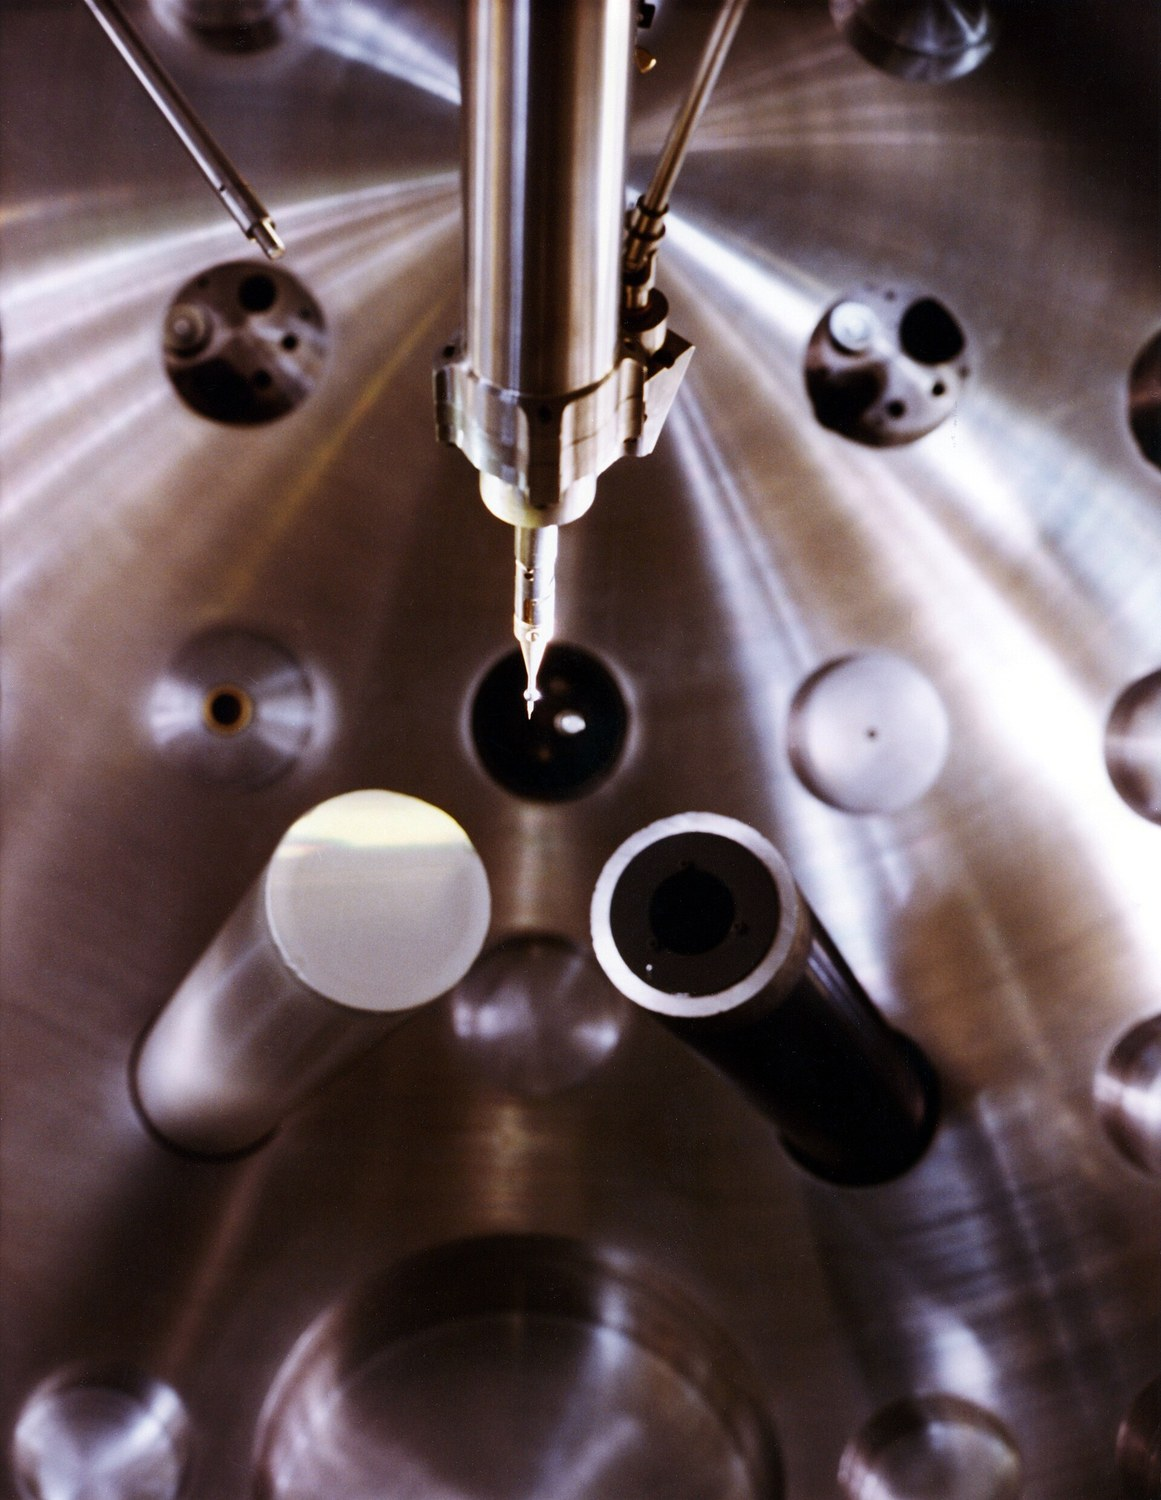
\includegraphics[width=0.69\textwidth]{../figures/y_shiva_chamber.jpg}
\caption{Shiva 靶室：把几十束激光聚到一点的那个房间。相对论透明讲的是激光把固体电离成等离子体的那一步；在实验室里，这一步发生在一个被几十束激光同时照到的靶点上。}
\label{fig:photo-appy2}
\figsource{Lawrence Livermore National Laboratory，Public domain（Wikimedia Commons）}
\end{figure}

\section{相对论透明：强激光怎么把固体变成等离子体}
\label{sec:app-y-transparency}

尾场加速用的是稀薄等离子体（$n_e = 10^{18}\ \mathrm{cm^{-3}}$）。
把同一束激光打到\textbf{固体}上会怎样？固体的电子密度是
$n_e = 10^{23}\ \mathrm{cm^{-3}}$，比临界密度高得多，
按线性理论激光根本进不去，只会被表面反射。

但强场改变了判据。电子质量变成 $m_e\gamma$ 之后，临界密度也跟着变成 $\gamma n_c$：
\begin{equation}
n_{c,\mathrm{rel}} = \gamma\, n_c = 8.42065\times10^{28}\ \mathrm{m^{-3}},
\label{eq:app-y-transparent}
\end{equation}
$\gamma = 48.3401$（式 \eqref{eq:app-y-up}）。于是\textbf{相对论透明}条件写成
\begin{equation}
a_0 > \frac{n_e}{n_c}.
\label{eq:app-y-itr}
\end{equation}
固体靶的 $n_e/n_c = 57.40661$，本工作点 $a_0 = 68.3486$，
余量 $1.19061$——\textbf{刚刚过线，只多出 $19\%$}。
对应的阈值强度是 $7.05447\times10^{21}\ \mathrm{W\,cm^{-2}}$，
比本工作点只低 $1.41754$ 倍。这个「刚刚好」不是巧合：
现代强场实验就是把强度选在透明阈值附近，因为只有在这个窗口里，
激光才能既进入过密等离子体、又不至于把它完全推开。

\begin{table}[htbp]
\centering
\small
\begin{tabular}{p{3.4cm}p{3.3cm}p{3.5cm}p{3.1cm}}
\toprule
量 & 数值 & 与工作点的关系 & 含义 \\
\midrule
固体 $n_e/n_c$ & $57.40661$ & 透明所需的 $a_0$ 下限 & 线性理论下不透明 \\
工作点 $a_0$ & $68.3486$ & 余量 $1.19061$ & 刚过线，只多 $19\%$ \\
阈值强度 & $7.05447\times10^{21}\ \mathrm{W\,cm^{-2}}$ & 低 $1.41754$ 倍 & 实验窗口就在附近 \\
相对论临界密度 & $8.42065\times10^{28}\ \mathrm{m^{-3}}$ & $= \gamma n_c$ & 质量变大抬高了 $n_c$ \\
\bottomrule
\end{tabular}
\caption{相对论透明。第二行是本节最值得记住的一句：
\textbf{透明不是把靶打薄了，而是把电子的质量变大了}。}
\label{tab:app-y-transparency}
\end{table}

\begin{tip}{透明不等于穿透}{tip-app-y-transparency}
「相对论透明」这个词容易误导：它不是说激光像穿过玻璃一样穿过去，
而是说\textbf{等离子体对激光的折射率被电子的相对论质量改写了}。
式 \eqref{eq:app-y-transparent} 里唯一变化的量是 $\gamma$——
密度没变、靶没变、激光波长没变，变的只是「电子的惯性」。
理解这一点，就能理解为什么相对论透明需要\textbf{极高的瞬时强度}：
一旦激光过去，$\gamma$ 立刻回到 $1$，透明窗口就关上了。
\end{tip}

{\footnotesize
\textbf{出处：}相对论透明的判据参照 Gibbon \emph{Short Pulse Laser Interactions
with Matter}（2005）第 5 章与 Kaw \& Dawson（1970）\emph{Phys.\ Fluids}
\textbf{13}, 472。
把 $\gamma n_c$ 作为有效临界密度的写法见 Esarey 等（2009）
\emph{Rev.\ Mod.\ Phys.} \textbf{81}, 1229。
}

\section{辐射压强与 QED 参数：离 Schwinger 场还有多远}
\label{sec:app-y-qed}

强激光不只是把电子加速，它还\textbf{推}物质。光子带着动量，动量流就是压强：
\begin{equation}
\frac{I}{c} = 3.33564\times10^{17}\ \mathrm{Pa}
= 3.3356\times10^{12}\ \mathrm{bar}\;(3.3356\times10^{6}\ \mathrm{Mbar}),
\label{eq:app-y-pressure}
\end{equation}
如果被完全反射，压强加倍：$2I/c = 6.67128\times10^{17}\ \mathrm{Pa}$。
把这个数与托卡马克的磁压比一下（附录 S 口径，$B = 5.3\ \mathrm{T}$ 对应
$B^2/(2\mu_0) = 1.11767\times10^{7}\ \mathrm{Pa}$）：
\begin{equation}
\frac{I/c}{B^2/(2\mu_0)} = 2.9845\times10^{10}.
\label{eq:app-y-chi}
\end{equation}
\textbf{三百亿倍}。所以激光等离子体不是「另一个托卡马克」，
而是把同一套等离子体物理放在一个压强高十个数量级的箱子里。
这也是为什么惯性约束（Y.6）要靠\textbf{内爆}而不是靠\textbf{约束}：
压强只存在几十皮秒，唯一能利用它的方式是让物质在这么短的时间里来不及散开。

第二个量是电子的\textbf{量子非线性参数}，它衡量电子在它的静止系里看到的场
离 Schwinger 场有多远：
\begin{equation}
\chi = \gamma\,\frac{E_L}{E_S} = 0.0100206,
\qquad
\frac{1}{\chi} = 99.794.
\label{eq:app-y-ratio2}
\end{equation}
$\chi$ 约等于百分之一。这个百分之一的量级很关键：
$\chi\ll1$ 时电子只是被加速；$\chi\sim1$ 时它开始一边运动一边辐射，
辐射反作用（radiation reaction）开始改写轨道；再往上就进入非线性 QED，
出现正负电子对。本工作点\textbf{离这三个门槛都还差一个到两个数量级}，
所以本附录只做经典计算——这不是简化，而是\textbf{如实标明适用边界}。

\begin{table}[htbp]
\centering
\small
\begin{tabular}{p{3.2cm}p{3.6cm}p{3.3cm}p{3.2cm}}
\toprule
量 & 数值 & 参照物 & 含义 \\
\midrule
辐射压强 $I/c$ & $3.33564\times10^{17}\ \mathrm{Pa}$ & 磁压 $1.11767\times10^{7}\ \mathrm{Pa}$ & 高 $2.9845\times10^{10}$ 倍 \\
反射加倍 $2I/c$ & $6.67128\times10^{17}\ \mathrm{Pa}$ & --- & 靶面受到的冲量 \\
QED 参数 $\chi$ & $0.0100206$ & $\chi=1$ 为 QED 门槛 & 还差约两个数量级 \\
$I/I_S$ & $4.30282\times10^{-8}$ & $I_S = 2.32406\times10^{33}\ \mathrm{W\,m^{-2}}$ & 离对产生更远 \\
\bottomrule
\end{tabular}
\caption{压强与 QED 参数。第三行的 $\chi$ 是本附录最需要「如实声明」的一个数：
它决定了经典计算在哪里失效，而本书不去猜失效之后的事。}
\label{tab:app-y-qed}
\end{table}

\begin{tip}{离 QED 门槛还差两个数量级，所以经典计算够用}{tip-app-y-qed}
表 \ref{tab:app-y-qed} 的 $\chi=0.0100206$ 是本附录的「适用边界声明」。
$\chi$ 量的是电子在自身静止系里看到的场与 Schwinger 场之比：
它到 $1$ 还差 $99.794$ 倍，所以本附录用经典电动力学算轨道是对的；
但也不能说「量子效应可以忽略」——$\chi\sim10^{-2}$ 已经足够让同步辐射阻尼
进入电子的运动方程，只是这一项在本附录的能量尺度上还不是主角。
\textbf{把「够用」与「可以忽略」分开写，是这一节唯一想留给读者的话。}
\end{tip}

\begin{tip}{光压比磁压大三百亿倍，但冲量才是可比的}{tip-app-y-pressure}
看到 $2.9845\times10^{10}$ 这个倍数，容易得出「激光等离子体比磁约束强得多」的结论。
这是把\textbf{压强}与\textbf{冲量}搞混了。托卡马克的磁压可以持续几千秒，
激光的辐射压只持续 $30\ \mathrm{fs}$（$3\times10^{-14}\ \mathrm{s}$）。
把压强乘上时间，两者的比就掉到 $10^{6}$ 量级；再乘上作用面积，
才是真正决定「能不能把物质压到一起」的那个数。
\textbf{比压强之前先问一句：它存在多久？}
\end{tip}

{\footnotesize
\textbf{出处：}辐射压与有质动力压强的量级参照 Gibbon \emph{Short Pulse Laser
Interactions with Matter}（2005）第 2 章。
量子非线性参数 $\chi$ 的定义与
$\chi\sim1$ 的物理含义参照 Ritus（1985）\emph{J.\ Sov.\ Laser Res.} \textbf{6}, 497
与 Mourou 等（2006）\emph{Rev.\ Mod.\ Phys.} \textbf{78}, 309。
托卡马克磁压沿用附录 S 口径。
}

\section{惯性约束：面密度、燃耗与增益}
\label{sec:app-y-icf}

强场的最后一个用途是把燃料\textbf{压缩}到聚变条件。惯性约束的核心判据不是温度、
不是密度，而是\textbf{面密度} $\rho R$——因为 DT 反应的产物（$3.5\ \mathrm{MeV}$
的 alpha 粒子，见附录 W）必须在燃料里停下来才能把能量留下。
取工程上常引用的目标值 $\rho R = 3\ \mathrm{g\,cm^{-2}} = 30\ \mathrm{kg\,m^{-2}}$，
压缩密度 $\rho = 200\ \mathrm{g\,cm^{-3}}$，于是燃料球的半径是
\begin{equation}
R = \frac{\rho R}{\rho} = 150\ \mathrm{\mu m},
\label{eq:app-y-rhor}
\end{equation}
体积 $V = 1.41372\times10^{-11}\ \mathrm{m^3}$，质量 $m = 2.8274\ \mathrm{mg}$。
\textbf{两毫克燃料，半径一百五十微米}——这就是一个点火靶的全部。

燃烧份额由面密度决定（这是\textbf{声明的}工程拟合，本书只用它的形状）：
\begin{equation}
f = \frac{\rho R}{\rho R + 6\ \mathrm{g\,cm^{-2}}} = 33.333\%.
\label{eq:app-y-burn}
\end{equation}
取 DT 比能 $3.396\times10^{14}\ \mathrm{J\,kg^{-1}}$（\textbf{声明值}），
总聚变能 $E_{\mathrm{fus}} = 960.2\ \mathrm{MJ}$，实际释放
$E_{\mathrm{burn}} = f E_{\mathrm{fus}} = 320.07\ \mathrm{MJ}$。若驱动器能量
$E_{\mathrm{drv}} = 2\ \mathrm{MJ}$，靶增益
\begin{equation}
G = \frac{E_{\mathrm{burn}}}{E_{\mathrm{drv}}} = 160.03273.
\label{eq:app-y-gainicf}
\end{equation}
$G = 160$ 听起来很高，但驱动器不是免费的：若驱动器效率 $10\%$，
墙插增益只有 $16.0033$。\textbf{把 $160$ 除以 $10$ 的那一步，
是惯性约束工程上最贵的一步}——这也是为什么激光器效率与靶增益同样重要。

\begin{table}[htbp]
\centering
\small
\begin{tabular}{p{3.2cm}p{3.2cm}p{3.4cm}p{3.4cm}}
\toprule
量 & 数值 & 由什么决定 & 备注 \\
\midrule
面密度 $\rho R$ & $3\ \mathrm{g\,cm^{-2}}$ & 工程目标 & alpha 粒子能否自吸收 \\
半径 $R$ & $150\ \mathrm{\mu m}$ & $\rho R/\rho$ & 压缩到 $\rho = 200\ \mathrm{g\,cm^{-3}}$ \\
燃料质量 & $2.8274\ \mathrm{mg}$ & $V\rho$ & 两毫克 \\
聚变能 $E_{\mathrm{fus}}$ & $960.2\ \mathrm{MJ}$ & $m\times3.396\times10^{14}$ & 声明比能 \\
燃烧份额 $f$ & $33.333\%$ & $\rho R/(\rho R+6)$ & 三分之一的燃料参与 \\
实际释放 & $320.07\ \mathrm{MJ}$ & $fE_{\mathrm{fus}}$ & 靶增益 $160.03273$ \\
\bottomrule
\end{tabular}
\caption{一个 $\rho R = 3\ \mathrm{g\,cm^{-2}}$ 点火靶的全部账。第四行与第五行含两个
\textbf{声明值}（DT 比能、燃耗拟合里的 $6\ \mathrm{g\,cm^{-2}}$），
它们不参与本书自拟的推导，只用来把量级说清楚。}
\label{tab:app-y-icf}
\end{table}

\begin{tip}{本附录不给实验点，只给标度律}{tip-app-y-honest}
强场物理是实验主导的领域，参数点极其分散：同样的强度，不同装置、不同脉宽、
不同对比度会给出完全不同的结果。所以本附录刻意\textbf{不给任何「实验结果对照表」}，
只给可以手算的标度律（$a_0$、$\lambda_p$、$L_d$、$\rho R$、$G$）与它们的适用边界。
凡是本书不能从第一原理复算的量——自聚焦系数 $17.4\ \mathrm{GW}$、
DT 比能 $3.396\times10^{14}\ \mathrm{J\,kg^{-1}}$、燃耗拟合里的 $6\ \mathrm{g\,cm^{-2}}$——
都在正文与表里写明是\textbf{声明值}。\textbf{把做不到的地方标出来，
比用一个看起来精确的数字盖过去更有用}——这是附录 V 立下的口径，这里是第三次。
\end{tip}

{\footnotesize
\textbf{出处：}面密度判据与燃耗份额的物理图像参照 Atzeni \& Meyer-ter-Vehn
\emph{The Physics of Inertial Fusion}（2004，第 1、3 章）与 Freidberg
\emph{Plasma Physics and Fusion Energy}（2007，第 14 章）。
alpha 粒子在燃料中的射程与自吸收口径与附录 W 一致。
}

\section{估算练习}
\label{sec:app-y-problems}

\textbf{练习 1} 若把强度降到 $10^{20}\ \mathrm{W\,cm^{-2}}$（波长不变），
$a_0$、$U_p$、$E_L$ 各是多少？$a_0$ 小了十倍，$U_p$ 是否也小了十倍？

\textbf{练习 2} 若把背景密度降到 $n_e = 10^{17}\ \mathrm{cm^{-3}}$，
波破场 $E_{WB}$、等离子体波长 $\lambda_p$、失相长度 $L_d$ 各变成多少？
加速梯度与加速距离朝相反方向变，总体增益是升还是降？

\textbf{练习 3} 若改用 $\mathrm{CO_2}$ 激光（$\lambda = 10.6\ \mathrm{\mu m}$），
临界密度 $n_c$ 变成多少？在同一密度 $n_e = 10^{18}\ \mathrm{cm^{-3}}$ 下，
$n_e/n_c$ 与失相长度 $L_d$ 变成多少？

\textbf{练习 4} 要让 $a_0 = 1$，需要多高的强度？在同样的焦斑面积下，
激光功率与脉冲能量各是多少？与工作点相比小了多少倍？

\textbf{练习 5} 固体靶的相对论透明阈值对应的强度是多少？
它比工作点低多少倍？对应的激光功率是多少？

\textbf{练习 6} 若把点火靶的目标降到 $\rho R = 1\ \mathrm{g\,cm^{-2}}$、
压缩密度降到 $100\ \mathrm{g\,cm^{-3}}$，半径、质量、总聚变能、
燃烧份额、实际释放与靶增益各是多少？

\textbf{解答 1} $a_0\propto\sqrt{I}$，所以
$a_0 = 6.83486$；$E_L = a_0 m_e\omega c/e = 2.74309\times10^{13}\ \mathrm{V\,m^{-1}}$；
$U_p = 2.01096\ \mathrm{MeV}$。\textbf{要点}：强度降 $100$ 倍，
$U_p$ 只降到 $1/12.0295$——因为 $\gamma$ 饱和了。
在 $a_0\gg1$ 的区间里 $U_p\approx m_ec^2a_0/\sqrt{2}$，
是\textbf{线性}而不是平方关系；只有 $a_0\ll1$ 时才是 $U_p\propto I$。
这就是为什么「强场」不能用微扰论来理解。

\textbf{解答 2} $E_{WB}\propto\sqrt{n_e}$，所以
$E_{WB} = 30.4082\ \mathrm{GV\,m^{-1}}$（比 $10^{18}$ 小 $3.1623$ 倍）；
$\lambda_p = 105.6\ \mathrm{\mu m}$；
$L_d = \lambda_p n_c/n_e = 1.8393\ \mathrm{m}$。
\textbf{要点}：梯度降 $3.1623$ 倍、距离涨 $31.623$ 倍（$L_d\propto n_e^{-3/2}$），
所以\textbf{增益涨十倍}（$5.5929\to$ 约 $55.9\ \mathrm{GeV}$）。
但距离涨到米级，装置不再「台式」——这就是失相长度与梯度的矛盾
（见 Y.3 的提示盒）。

\textbf{解答 3} $n_c\propto\lambda^{-2}$，所以
$n_c = 9.9222\times10^{18}\ \mathrm{cm^{-3}}$，
$n_e/n_c = 0.100784$；失相长度
$L_d = 0.3313\ \mathrm{mm}$，比 $0.8\ \mathrm{\mu m}$ 的情形短
$175.5625$ 倍。\textbf{要点}：长波长激光的临界密度低，
所以它的加速距离是毫米而不是厘米——$\mathrm{CO_2}$ 激光适合做单级低能、
高重复频率的加速，不适合做单级高能。

\textbf{解答 4} $a_0 = 1$ 对应
$I = 2.14063\times10^{18}\ \mathrm{W\,cm^{-2}}$；
在同一焦斑面积下 $P = 1.68124\times10^{12}\ \mathrm{W} = 1.68124\ \mathrm{TW}$、
$E = 50.44\ \mathrm{mJ}$。\textbf{要点}：与工作点相比，
强度小 $4671.5$ 倍、能量也小 $4671.5$ 倍（因为 $E\propto I$）。
这个量级正是现代桌面飞秒激光器的指标——\textbf{「相对论强场」并不需要巨型装置}。

\textbf{解答 5} 透明阈值 $a_0 = 57.4066$，对应
$I = 7.05447\times10^{21}\ \mathrm{W\,cm^{-2}}$，
比工作点低 $1.41754$ 倍；对应功率
$P = 5.54057\times10^{15}\ \mathrm{W} = 5540.6\ \mathrm{TW}$。
\textbf{要点}：本工作点比透明阈值只高一倍多，说明\textbf{它本来就在透明窗口附近}——
这是刻意选的：只有在这个窗口里，激光才能既进入过密区、又不完全推开它。

\textbf{解答 6} $R = \rho R/\rho = 100\ \mathrm{\mu m}$，
$m = 0.41888\ \mathrm{mg}$，$E_{\mathrm{fus}} = 142.25\ \mathrm{MJ}$，
$f = 14.286\%$，$E_{\mathrm{burn}} = 20.322\ \mathrm{MJ}$，
$G = 10.16081$。\textbf{要点}：面密度从 $3$ 降到 $1$，
燃烧份额从 $33.333\%$ 掉到 $14.286\%$（$f$ 不是线性下降），
靶增益从 $160.03273$ 掉到 $10.16081$——\textbf{降了将近十六倍}。
所以 $\rho R$ 是惯性约束里最不能省的参数。

\section{来源、分级与版权说明}
\label{sec:app-y-source}

\begingroup\small
本附录按难度分三档：Y.1 与 Y.2 是刻度与判据（读完应当能判断「一束激光算不算强场」）；
Y.3 与 Y.4 是两个具体算法（读完应当能独立复算尾场增益与透明阈值）；
Y.5 与 Y.6 是把强场放回能量账（读完应当能说清「激光等离子体与磁约束差在哪、
为什么惯性约束只能靠内爆」）。练习 1--6 都只需要本附录的公式与表，不需要查外部数据。

\begin{table}[htbp]
\centering
\small
\begin{tabular}{p{3.4cm}p{5.6cm}p{3.6cm}}
\toprule
本附录内容 & 借鉴来源 & 在本书里的位置 \\
\midrule
强场归一化振幅与有质动力势 &
Gibbon \emph{Short Pulse Laser Interactions with Matter}（2005）第 1、2 章 &
本附录 Y.1 \\
Schwinger 场与 QED 门槛 &
Schwinger（1951）\emph{Phys.\ Rev.} \textbf{82}, 664；Ritus（1985）\emph{J.\ Sov.\ Laser Res.} \textbf{6}, 497 &
本附录 Y.1、Y.5 \\
尾场加速与失相长度 &
Tajima \& Dawson（1979）\emph{Phys.\ Rev.\ Lett.} \textbf{43}, 267；Esarey 等（2009）\emph{Rev.\ Mod.\ Phys.} \textbf{81}, 1229 &
本附录 Y.2、Y.3 \\
自聚焦与相对论透明 &
Kaw \& Dawson（1970）\emph{Phys.\ Fluids} \textbf{13}, 472；Gibbon（2005）第 5 章 &
本附录 Y.4 \\
惯性约束面密度与燃耗 &
Atzeni \& Meyer-ter-Vehn \emph{The Physics of Inertial Fusion}（2004）第 1、3 章 &
本附录 Y.6；alpha 射程见附录 W \\
强场综述与实验现状 &
Mourou 等（2006）\emph{Rev.\ Mod.\ Phys.} \textbf{78}, 309 &
本附录 Y.1、Y.5 \\
\bottomrule
\end{tabular}
\caption{本附录的借鉴来源与对应位置。只借鉴物理结论、公式形式与题型；
全部数值、表格与文字自拟并由仓库脚本复算。}
\label{tab:app-y-source}
\end{table}

版权与复现口径，四条：第一，\textbf{不复制}任何教材或论文的表格数值，
表 \ref{tab:app-y-scales} 到表 \ref{tab:app-y-source} 的每一个数字都由
\texttt{tools/\allowbreak{}calc/\allowbreak{}appY\_calc.py} 在给定工作点上现算；第二，\textbf{不复制}原书的题面与解答文字，
练习 1--6 的题目与解答均为本书自拟；第三，\textbf{不复制}无法核验的 DOI 编号，
一律只给书名、作者、年份、卷期页；第四，\textbf{不复制}任何未经复算的「精确值」——
凡本附录引入的\textbf{声明值}（自聚焦系数 $17.4\ \mathrm{GW}$、
DT 比能 $3.396\times10^{14}\ \mathrm{J\,kg^{-1}}$、
燃耗拟合常数 $6\ \mathrm{g\,cm^{-2}}$、实验对照 $3.3\ \mathrm{cm}$）
都在正文里写明是量级值或文献报道值，不假装精确。
\endgroup
